\documentclass[12pt]{article}

\usepackage[utf8]{inputenc}
\usepackage{amsmath}
\usepackage{amssymb}
\usepackage{caption}
\usepackage{color}
\usepackage{float}
\usepackage{graphicx}
\usepackage{listings}
\usepackage{physics}

\title{
	\Large{CSE-300 Assignment-1}
	\endgraf
	\Large{Introduction to \LaTeX}
	\endgraf\bigskip	
	\textbf{An Introduction To Dynamic Programming Algorithms}
	\endgraf\bigskip
}

\author{
	\Large{Waqar Hassan Khan}\\
	\Large{Student ID : 1505107}
}

\date{}

\begin{document}

%--------------------------------------------------cover page	
\maketitle

\section*{}
\begin{figure}[b]
	\centering
	
	\captionsetup{justification=centering}
	
\includegraphics[width = 0.1\textwidth]{image/buet.png}
	\caption*{
		\Large{Department of Computer Science and Engineering}
		\\
		\Large{Bangladesh University of Engineering and Technology}
		\\
		\Large{(BUET)}
		\\
		\Large{Dhaka 1000}
		\\
		\Large{\today}
	}
	
\end{figure}
%--------------------------------------------------cover page

\newpage
\tableofcontents
\newpage

%--------------------------------------------------intro
\section{Introduction}
In the world of computer programming techniques \textbf{Dynamic Programming} a.k.a \textcolor{blue}{\textit{DP}} perhaps is the most important one used in various fields of computer science. When i came by the name i thought it was something that have difficult mathematical equation like the equation-
\begin{equation*}
e ^ x = 1 + x + \frac{x ^ 2}{ 2 !} + \frac{x ^ 3}{3!} + \cdot \cdot \cdot ~ \infty
\label{eqn:e}
\end{equation*}  
\newline
or like the equation $\pdv[2]{\psi}{x}+\dfrac{8\pi^2m}{\hslash^2}(E-V)\psi$
\newline

But it is really a different thing.The word was first used by \textcolor{blue}{\textbf{Bellman}}. Dynamic Programming is an algorithmic paradigm that solves a given complex problem by breaking it into subproblems and stores the results of subproblems to avoid computing the same results again. Following are the two main properties of a problem that suggest that the given problem can be solved using Dynamic programming.

\begin{itemize}
	\item Overlapping Subproblems
	\item Optimal Substructure
\end{itemize}

\subsection{Overlapping Subproblems}
The subproblems of a problem may overlap while solving using \textbf{Divide and Conquer}, that is we may end solving the same thing over and over again. In DP we keep track of the solved sub-problems and avoid solving them more than once. Once solved it is stored to use for farther use.
\begin{figure}[H]
	\centering
	\captionsetup{justification=centering}
	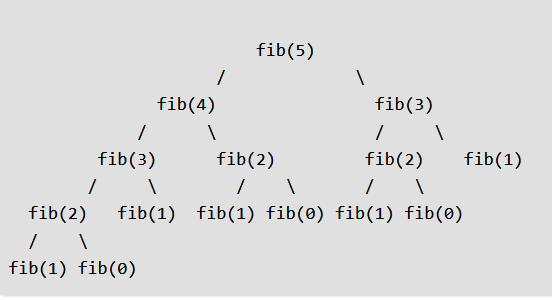
\includegraphics[width = 0.5\textwidth]{image/overlap.png}
	\caption{
		Overlapping Subproblems in determination of Fibonacci series
	}
	\label{fig:fib}
	
\end{figure}

\subsection{Optimal Sub-structure}
 A given problems has Optimal Substructure Property if optimal solution of the given problem can be obtained by using optimal solutions of its subproblems.
For example, the Shortest Path problem has following optimal substructure property:
If a node x lies in the shortest path from a source node u to destination node v then the shortest path from u to v is combination of shortest path from u to x and shortest path from x to v. The standard All Pair Shortest Path algorithms like Floyd–Warshall is an example of Dynamic Programming
%--------------------------------------------------intro

%--------------------------------------------------section-two
\section{Solving a DP}
Steps to solve a DP:
	\begin{enumerate}
		\item Identify if it is a DP problem
		\item Decide a state expression with least parameters
		\item Formulate state relationship    
		\item Do tabulation (or add memoization)
		
	\end{enumerate}

	\begin{description}
		\item[Tabulation] Bottom Up Dynamic Programming (starting from dp[0] we move up) 
		\item[Memoization] Top Down Dynamic Programming (starting from dp[n] we use recursion here)
	\end{description}
%--------------------------------------------------section-two

%--------------------------------------------------some ilustrated example
\section{Some Solved Problems}
\subsection{Fibonacci Numbers}
The Fibonacci series is as follows 1 1 2 3 5 8 13 21...
We have to write a program that can give us nth Fibonacci number. We can use both approach,
first we show bottom-up then top-down. The codes are written in python-3\newline
(Please see Figure \ref{fig:fib}) 
\subsubsection{top-down approach}
\begin{lstlisting}[language=python]
	
	#bottom-up
	n=int(input())
	
	fib=[None]*(n+1)
	
	#base case
	fib[1]=fib[2]=1
	for i in range(3,n+1):
		fib[i]=fib[i-1]+fib[i-2]
	
	print(fib[n])
\end{lstlisting}


\subsubsection{bottom-up approach}
\begin{lstlisting}[language=python]

	def fibonacci(n):
		if fib[n]>0:
			return fib[n]
		
		if n==1 or n==2:
			return 1
		
		fib[n]=fibonacci(n-1)+fibonacci(n-2)
		return fib[n]
	
	#top-down
	n=int(input())
	fib=[0]*(n+1)
	
	print(fibonacci(n))
\end{lstlisting}

\subsection{Calculating $^nC_r$}
Calculating $^nC_r$ using dynamic programming is really easy. We have to use the recurrence relation  $^nC_r=^n^-^1C_r+^n^-^1C_r_-_1$

\begin{figure}[H]
	\centering
	
	\captionsetup{justification=centering}
	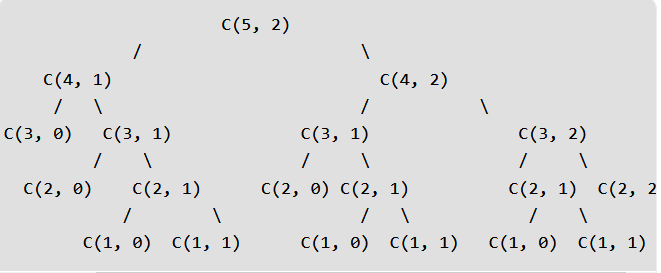
\includegraphics[width = 0.5\textwidth]{image/ncr.png}
	\caption{
		Overlapping Subproblems in determination of Fibonacci series
	}
	
\end{figure}

\begin{lstlisting}[language=python]
	
	def nCr(n,r):
		if n==0:
			return 0
		
		if r==0 or r==n:
			return 1
		
		dp[n][r]=nCr(n-1,r)+nCr(n-1,r-1)
			return dp[n][r]
	
	#top-down
	n,r=map(int,input().split())
	dp=[[0]*(r+1)]*(n+1)
	
	print(nCr(n,r))
	
\end{lstlisting}
%--------------------------------------------------some ilustrated example

\section{Conclusion}
Dynamic Programming has many classic problems and other problems need intuition and practice to solve.

\end{document}


